\documentclass[12pt,a4paper]{article}

\usepackage{fancyvrb,subfloat,amsthm,amssymb,mathrsfs,setspace,mathtools,amsmath}%amsmath, latexsym,footmisc
\usepackage[T1]{fontenc}
\usepackage{lmodern}
\usepackage{hyperref}
% \usepackage{pstcol}
% \usepackage{play}
\usepackage{fontenc,graphicx,caption,epsfig,subfig,float}
%\usepackage[grey,times]{quotchap}
\usepackage[nottoc]{tocbibind}
\usepackage[square,authoryear]{natbib}
%\renewcommand{\chaptermark}[1]{\markboth{#1}{}}
\renewcommand{\sectionmark}[1]{\markright{\thesection\ #1}}
%
%\setcitestyle{authoryear}
\input xy
\xyoption{all}


\theoremstyle{plain}
\newtheorem{theorem}{Theorem}[section]
\newtheorem{lemma}[theorem]{Lemma}
\newtheorem{corollary}[theorem]{Corollary}
\newtheorem{proposition}[theorem]{Proposition}

\theoremstyle{definition}
\newtheorem{definition}[theorem]{Definition}
\newtheorem{example}[theorem]{Example}
\newtheorem{notation}[theorem]{Notation}
\newcommand{\norm}[1]{\left\lVert#1\right\rVert}
\theoremstyle{remark}
\newtheorem{remark}[theorem]{Remark}
\renewcommand{\baselinestretch}{1.5}
\usepackage[margin=0.75in]{geometry}


\begin{document}


% --------------- Title page -----------------------

\begin{titlepage}
\enlargethispage{3cm}

\begin{center}

\vspace*{0.5cm}

\textbf{\Large Titanic: Machine Learning from Disaster (Kaggle)}\\[2cm]


{\large \emph{by}}\\[5pt]
{\large\bf {Mayank Sardana}}\\[1pt]
{\large (mas613@pitt.edu)}\\
{\large\bf {Dimple Varma}}\\[1pt]
{\large (ddv1@pitt.edu)}\\
{\large\bf {Charan Teja GR}}\\[1pt]
{\large (chg81@pitt.edu)}\\[2cm]

\end{center}

\end{titlepage}

\clearpage

\newpage



% =========== Main chapters starts here. Type in separate files and include the file name here. ==
% ============================

\pagenumbering{arabic}
\setcounter{page}{1}

\tableofcontents
\clearpage %\cleardoublepage %for openright
%\addcontentsline{toc}{chapter}{List of Figures}
\listoffigures
%\clearpage %\cleardoublepage %for openright
%\addcontentsline{toc}{chapter}{List of Tables}
\clearpage

\section{Introduction}
\vspace{-0.1in}
The sinking of Titanic is the most infamous shipwrecks and shocked the global world and led to better safety regulations for ships. The major reason was not enough lifeboats for passengers and crew. There was both luck in some people surviving but there were some statistics led results which showed some group survived more than other group. The project involved analyzing which class/category of people survived more than others. The heart of the problem lies in the question, which machine learning techniques is to be used for given training data to perform the predictive task which can help us find out the group of people that had more chances of survival over others.

We follow the concept of Exploratory Data Analysis (EDA) to start with getting insights into the training data. We try to extract as much information from various graphics as we can and infer useful information out of it. Python and R, both being computationally strong language are used during the project work. We first try to deduce as much information as we can from the various plots as explained in the next section. Further we used different models to perform the prediction task and come with a good accuracy. We discuss the procedure along with the results in a detailed manner in the following paragraphs.

%\section{Literature Review}
\vspace{-0.1in}
This section discusses the work that has been done in this field and the way it has been done. The area of analytics and its application in the field of movies has not been explored much especially the one based on sentiment analysis of public opinion due to the non-availability of large chunks of data until few years back. However, some key findings as discussed below have made a significant impact on the film industry.

The initial piece of work was done to find a correlation between the box-office data and the tweets from Twitter using simple linear regression. \citet{asur2010predicting} discusses some of the regression techniques implemented for predicting the box-office revenue. Time stamped data of tweets was collected for around 84 movies over a span of 3-4 months which included around 10 million tweets. The author initially calculated the rate at which tweets were posted in different time intervals when the topic relating to movie was trending. Linear regression model was applied to fit in different pairs of data to predict the box-office revenue from the tweet rates in future. This served as the initial information for the prediction purpose. Next, the sentiment analysis of the tweets was done before and after the release of movie to see the change in the intensity of emotions which had clear affects on the revenue as well. The stronger the sentiments(positive/negative) on the day of the release and during the opening weekend, the sharper was the change (increase/decrease) in revenue. Furthermore, some movies which had lukewarm response in the opening week but had stronger display of emotions on social media displayed a sharp rise in their revenue in the weeks ahead of the release. 

\citet{sharda2006predicting} attempted to apply neural network based algorithm for prediction of box office revenue. The author used various features for this purpose which he further classified into independent and dependent variables. The features didn't include any public opinion/sentiments as an input variable rather all the features were related to the movie itself. The different features taken into account were Star Cast, Motion Picture Ratings, Genre, Competition, Sequel, Number of screens all of which were independent of each other and the Box-office Revenue as the only dependent variable. This was the first instance of the application of neural networks in the Film industry to predict the outcomes. The author used Multi-Layer Perceptron with 2 hidden layers for this purpose in which he assigned certain discrete values to each feature and corresponding numerical weight was also given. Further, he tested the performance of the neural network using the percent success rate which is the ratio of total correct classifications to total number of samples, averaged for all classes in the classification problem. This approach proved quite successful by giving the revenue of a movie as the function of various variables which helped a movie producer and director in selecting the crew members and planning out the release in way that can be profitable.

In another attempt at predicting the box-office revenue, \citet{moviemod} used a completely different approach at solving some unanswered questions relating to film industry. Markov chain was used for estimating the revenue based on the consumer behavior. The paper was published more than a decade back when there was no online social media platform for the prediction purpose. The states of the Markov change represented the behavioral states of a consumer about movie which included 'undecided', 'considerer', 'rejecter' etc. The change of state usually take place based on the movie related factors. The probability of moving from one state to other was calculated based on various factors that tend a consumer to form an impression about it. They took into account the most important factor that was key to the success/failure of a movie, vis-a-vis word-of-mouth which nowadays reflect on the social media platforms in the form of user's opinion. The results were significant if we see it relatively as there was no strong mode of communication at that point of time. 

\section{Exploratory Data Analysis}
\vspace{-0.1in}

Exploratory data analysis (EDA) is an approach to analyze data sets and summarize their main characteristics. EDA is used for extracting information and visualization of it without involving the formal modeling or hypothesis testing task. It is an approach for data analysis that employs a variety of techniques to
\begin{itemize}
\item Maximize insight into a data set
\item Detect outliers and anomalies
\item Uncover underlying structure
\item Extract important variables
\item Test underlying assumptions
\item Develop economical models
\item Determine optimal factor settings
\end{itemize}

Most EDA techniques involve graphical representations with a few quantitative models. The reason for the heavy reliance on graphics is to open-mindedly explore data sets and it gives the analysts exceptional power to do so. It is enticing to reveal its structural secrets, and being always ready to gain some new, often unsuspected, insight into the data.
The particular graphical techniques employed in EDA are often quite simple, consisting of various techniques of:

\begin{itemize}
\item Plotting the raw data with techniques such as data traces, histograms, bihistograms, probability plots, log plots, block plots.
\item Plotting simple statistics such as mean plots, standard deviation plots, box plots, and main effects plots of the raw data.
\item Positioning such plots so as to maximize our natural pattern-recognition abilities, such as using different colors and types of plots for one type of data.
\end{itemize}


\subsection{Dataset Characteristics}
The training dataset provided by Kaggle contained 12 attributes (columns) with 891 records. These attributes included \textit{PassengerId,Survived,Pclass,Name,Sex,Age,SibSp,Parch,Ticket,Fare,Cabin and Embarked}. Here is a short description about each of the attributes/variables:
\begin{itemize}
\item Survived: Passenger survival. Takes value 0 for No and 1 for Yes.
\item Pclass: Passenger Class. Takes value 1 for 1st, 2 for 2nd and 3 for 3rd
\item name: Passenger Name
\item sex: Passenger Gender. Takes value male and female.
\item age: Passenger Age. Continuous variable takes non negative values.
\item sibsp: Number of Siblings/Spouses Aboard. Takes positive integral values.
\item parch: Number of Parents/Children Aboard. Takes positive integral values.
\item ticket: Passenger Ticket number.
\item fare: Passenger ticket fare. Continuous variable takes non negative values.
\item cabin: Passenger Cabin.
\item embarked: Port of Embarkation. Takes value C = Cherbourg, Q = Queenstown and S = Southampton.
\end{itemize}

Here are some of the special notes provided by Kaggle:
\begin{enumerate}
\item Pclass is a proxy for socio-economic status (SES). 1st ~ Upper; 2nd ~ Middle; 3rd ~ Lower

\item Age is in Years; Fractional if Age less than One (1). If the Age is Estimated, it is in the form xx.5

\item With respect to the family relation variables (i.e. sibsp and parch) some relations were ignored.  The following are the definitions used for sibsp and parch.
\begin{enumerate}

\item[Sibling:]  Brother, Sister, Stepbrother, or Stepsister of Passenger Aboard Titanic
\item[Spouse:]   Husband or Wife of Passenger Aboard Titanic (Mistresses and Fiances Ignored)
\item[Parent:]   Mother or Father of Passenger Aboard Titanic
\item[Child:]    Son, Daughter, Stepson, or Stepdaughter of Passenger Aboard Titanic

\end{enumerate}
\item Other family relatives excluded from this study include cousins,nephews/nieces, aunts/uncles, and in-laws.  Some children travelled only with a nanny, therefore parch=0 for them.  As well, some travelled with very close friends or neighbors in a village, however, the definitions do not support such relations.

\end{enumerate}

\subsection{Missing Data Completion}
While doing initial analysis, we observed that, for some variables, a lot values are not reported or are missing. The variables include Age, Cabin, Fare and Embarked. The variable Age is one of the most crucial variables amongst those specified as it plays significant role in prediction task (as will be observed later). These type of missing data are Missing at Random and can be estimated using different techniques as discussed below:
\begin{itemize}
\item Dropping Variables: We begin with dropping the data records with missing values and try getting insights into the data by plotting graph. However, since the a significant number of records have missing age values (almost 20\%), this method further worsens the training set. But it works fine with Cabin as almost 50\% of records having missing cabin values which restricts application of any other data completion technique. Embarked and Fare have only 1-2 records missing which don't really affect classification accuracy to a significant extent.
\item Mean: For age values, we take the mean value of non-missing values of age variable and assign it to all the missing records. As expected, this performs better and improves the correlation between this and variable to be predicted. We can similarly do the same for Embarked and Fare also. However, the thing to be noted here is that Embarked is categorical variable and so we assign the missing record the value which occurs most often. Furthermore, as we will see in the following sections, fare variable is not normally distributed and assigning mean to the missing record can prove to be misleading.
\item Class-wise mean: For age values, we observed through initial analysis that males have higher average/mean age values compared to females. Therefore, we calculated 2 different mean values one each for male and female by using the same method as mentioned in last point. We then assign the male average ages to the missing records with sex value as male and same for the females. It may not have created a significant impact on the classification accuracy, but it is considered as a good practice and can impact the accuracy if the data set is large.
\item Linear Regression: We then used a more complex way to estimate the missing age values. We applied linear regression to get the age values. However, this method had one serious drawback. Some of the values estimated were negative which poses serious problems to classifier. We used Scikit-Learn library in Python to implement regression.
\item ANOVA: As suggested in the Tutorials for Random Forest, we followed this method of regression for estimating the missing age values and it did perform well on that part.
\end{itemize}
\subsection{Feature Extraction}
There are various features that are considered for the analysis of data set such as the passenger class, age, gender etc. We consider each of them separately as follows:

\begin{figure}
\centering
\begin{minipage}{.5\textwidth}
  \centering
  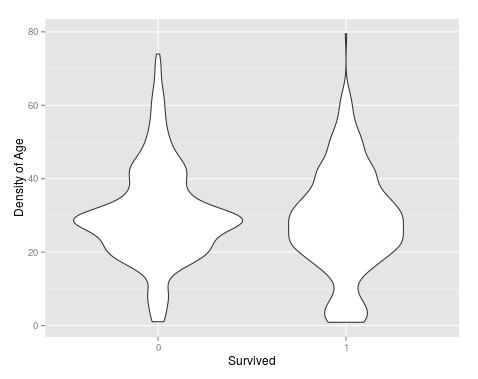
\includegraphics[width=1\linewidth]{figs/plot11}
  \captionof{figure}{Distribution of Age\\ in Survivors/Deaths}
  \label{fig:plot11}
\end{minipage}%
\begin{minipage}{.5\textwidth}
  \centering
  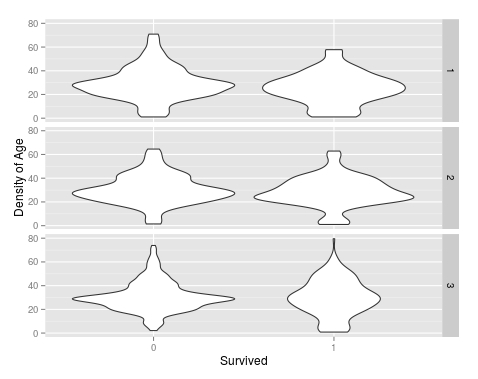
\includegraphics[width=1\linewidth]{figs/plot13}
  \captionof{figure}{Density of Age for Survivors/Deaths\\ in various classes (Voilin Plot)}
  \label{fig:plot13}
\end{minipage}
\end{figure}

\begin{figure}
\centering
\begin{minipage}{.5\textwidth}
  \centering
  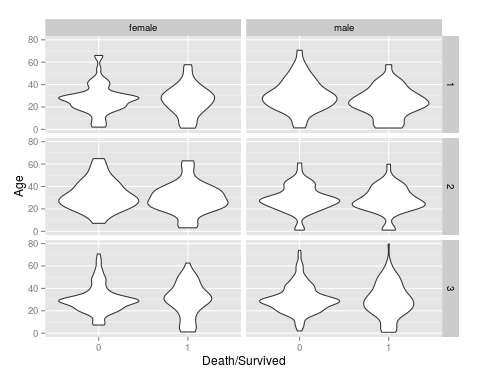
\includegraphics[width=1\linewidth]{figs/plot10}
  \captionof{figure}{Distribution of Age\\ for different Class and Gender}
  \label{fig:plot10}
\end{minipage}%
\begin{minipage}{.5\textwidth}
  \centering
  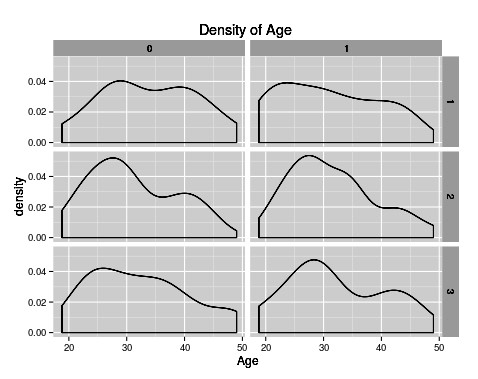
\includegraphics[width=1\linewidth]{figs/plot9}
  \captionof{figure}{Distribution of Middle Age(>20 \\and <50) Survivors/Deaths for different Class}
  \label{fig:plot9}
\end{minipage}
\end{figure}

\begin{figure}
\centering
\begin{minipage}{.5\textwidth}
  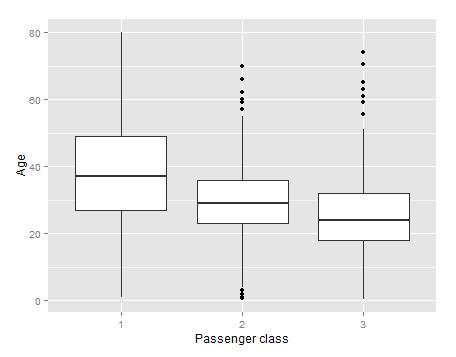
\includegraphics[width=1\linewidth]{figs/plot14}
  \captionof{figure}{Box plot for Passenger class vs Age}
  \label{fig:plot14}
\end{minipage}%
\begin{minipage}{.5\textwidth}
  \centering
  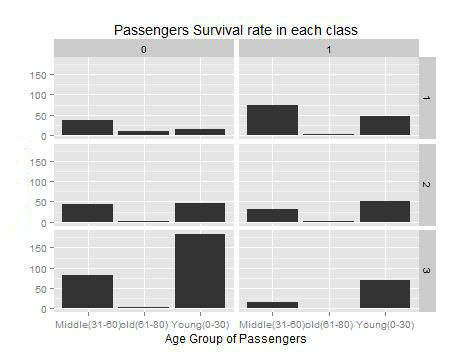
\includegraphics[width=1\linewidth]{figs/plot15}
  \captionof{figure}{Passenger Survivor for different\\ Age Groups and Class}
  \label{fig:plot15}
\end{minipage}
\end{figure}

We did some initial analysis of data as shown in the above Figures. Fig. \ref{fig:plot9},\ref{fig:plot10} \ref{fig:plot13} and \ref{fig:plot11} gave insights into the distribution of age seen from different angles. From these plots, we deduced that significant number of children(age<18) survived in Pclass 2 and 3. This helped in deciding one of the feature which is discussed in Random Forest model. Also, 1st and 2nd class senior citizens (age>50) were given preference as there are more survivors.

\begin{figure}
\centering
\begin{minipage}{.5\textwidth}
  \centering
  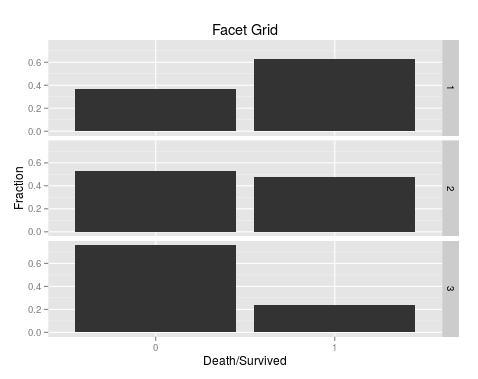
\includegraphics[width=1\linewidth]{figs/plot12}
  \captionof{figure}{Survivors/Deaths for different Pclass}
  \label{fig:plot12}
\end{minipage}%
\begin{minipage}{.5\textwidth}
  \centering
  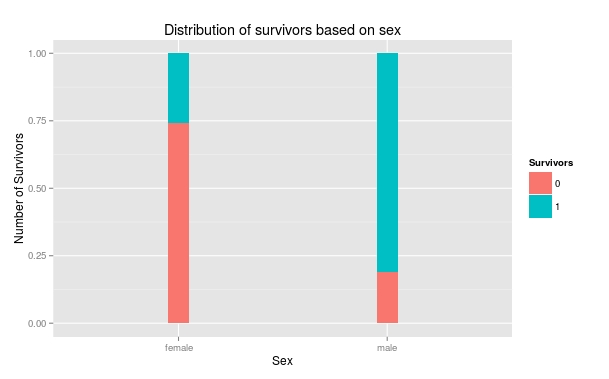
\includegraphics[width=1\linewidth]{figs/plot17}
  \captionof{figure}{Distribution of Survivors based\\ on Sex}
  \label{fig:plot17}
\end{minipage}
\end{figure}

\begin{figure}
\centering
\begin{minipage}{.5\textwidth}
  \centering
  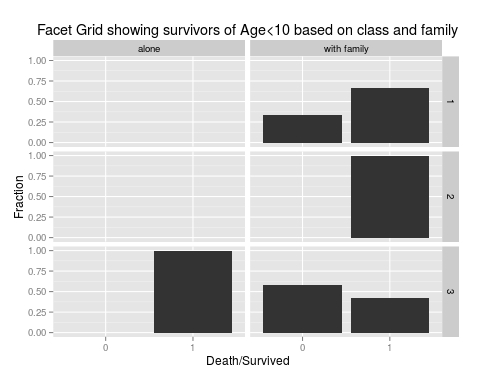
\includegraphics[width=1\linewidth]{figs/plot1}
  \captionof{figure}{Child(age<10) Survivors as\\ function of family and class}
  \label{fig:plot1}
\end{minipage}%
\begin{minipage}{.5\textwidth}
  \centering
  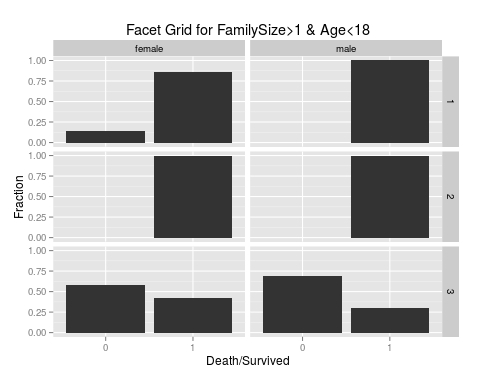
\includegraphics[width=1\linewidth]{figs/plot6}
  \captionof{figure}{Survivors as function of Family\\ and Age}
  \label{fig:plot6}
\end{minipage}
\end{figure}

Fig. \ref{fig:plot1} gave more insights into the child survivors when we saw its relationship with the family and class. As expected there were only a few children who were travelling alone. Almost all them were with family and their chances of survival also improved because of that. As can be seen, almost all of the 1st and 2nd class children survived the titanic crash.
Fig. \ref{fig:plot6} is one of the most crucial plot which helped us in improving the accuracy in Random Forest. This plot conveys that almost all the children(age<18) in 1st and 2nd class with familysize>1 survived the titanic crash.

\begin{figure}
\centering
\begin{minipage}{.5\textwidth}
  \centering
  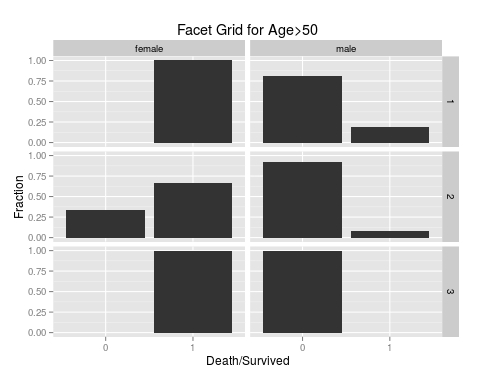
\includegraphics[width=1\linewidth]{figs/plot4}
  \captionof{figure}{Distribution of Survivors for\\ various class and Gender for\\ senior citizens (age>50)}
  \label{fig:plot4}
\end{minipage}%
\begin{minipage}{.5\textwidth}
  \centering
  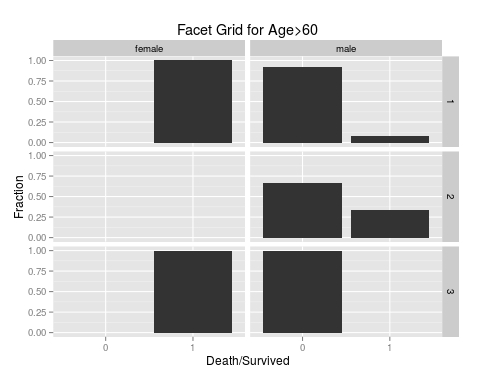
\includegraphics[width=1\linewidth]{figs/plot2}
  \captionof{figure}{Distribution of Survivors for\\ various class and Gender for\\ senior citizens (age>60)}
  \label{fig:plot2}
\end{minipage}
\end{figure}

Fig. \ref{fig:plot2} and \ref{fig:plot4} is in continuation with analysis done in various plots above. As can be seen from plot, almost all the females survived who have age>60 which was also one of our hypothesis as we know senior citizens were given preference. However, it is surprising to see that most of senior citizen males died. We extended the senior citizen age bar from 60 to 50 and it didn't have any significant difference.

\section{Machine Learning Models}
\vspace{-0.1in}

\subsection{Support Vector Machine}

\subsubsection{Introduction}
SVMs (Support Vector Machines) are a useful technique for data classification. A classification task usually involves separating data into training and testing sets. Each instance in the training set contains one "target value" (i.e. the class labels) and several "attributes" (i.e. the features or observed variables). The goal of SVM is to produce a model (based on the training data) which predicts the target values of the test data given only the test data attributes.

Here, training vectors $x_i$ are mapped into a higher (maybe infinite) dimensional space by the function $\phi$. SVM finds a linear separating hyperplane with the maximal margin in this higher dimensional space. C > 0 is the penalty parameter of the error term. Furthermore, $K(x_i ,x_j)$ is called the kernel function. Though new kernels are being proposed by researchers, beginners may find in SVM books the following four basic kernels:
\begin{itemize}

\item linear: $K(x_i , x_j) = x_i^\intercal x_j$.

\item polynomial: $K(x_i , x_j) = (\gamma\times(x_i^\intercal x_j+r))^d , \gamma > 0$.

\item radial basis function (RBF): $K(x_i,x_j) = \frac{1}{{e^(\gamma\times(norm(x_i-x_j)^2))}}, \gamma > 0$.

\item sigmoid: $K(x_i , x_j ) = tanh(\gamma\times(x_i^\intercal x_j) + r)$. Here, $\gamma$, r, and d are kernel parameters.
\end{itemize}

\subsubsection{Procedure}

We followed the following appproach to perform the classification with SVM:
\begin{itemize}

\item Transform data to the format of an SVM package

\item Conduct simple scaling on the data(if any)

\item Consider the RBF kernel in SVM package

\item Use cross-validation and grid search to find the best parameter C and $\gamma$

\item Use the best parameter C and $\gamma$ to train the whole training set.

\item Test
\end{itemize}

Scaling before applying SVM is very important. The main advantage of scaling is to avoid attributes in greater numeric ranges dominating those in smaller numeric ranges. In our data set, there were a lot of categorical variables which is not dealt by SVM. So, we first began with converting those variables to numbers so that it is compatible with SVMs. For this we used \textbf{onehot encoding} which refers to a group of bits among which the legal combinations of values are only those with a single high (1) bit and all the others low (0). For example, the Age took two values: male and female. We mapped male to [0,1] vector and female to [1,0] vector. We did the same for other variables as well. Now, the age and fare were the only continuous variables. There is no standard procedure for using it in SVMs. Mapping it to discrete vectors is one way and scaling it to lower values is another way. We used the first approach and therefore, formed groups for each of the variables based on the similarity in the group which was inferred from the exploratory analysis. \\

Secondly, we chose RBF kernel for classification purpose because of its various advantages. This kernel nonlinearly maps samples into a higher dimensional space so it, unlike the linear kernel, can handle the case when the relation between class labels and attributes is nonlinear. Another reason is the number of hyperparameters which influences the complexity
of model selection. The polynomial kernel has more hyperparameters than the RBF kernel.

Thirdly, we perform parameter estimation for RBF kernel using cross validation and grid search. There are two parameters for an RBF kernel: C and $\gamma$. It is not known beforehand
which C and $\gamma$ are best for a given problem. The goal is to identify good (C, $\gamma$) so that the classifier can accurately predict unknown data (i.e. testing data). We use cross validation for estimating the parameters along with grid search. In k-fold cross-validation, we first divide the training set into k subsets of equal size. Sequentially one subset is tested using the classifier trained on the remaining k − 1 subsets. Thus, each instance of the whole training set is predicted once so the cross-validation accuracy is the percentage of data which are correctly classified. For performing cross validation, we need parameter values. So, Various pairs of (C, $\gamma$) values are tried and the one with the best cross-validation accuracy is picked. We got to know that trying exponentially growing sequences of C and $\gamma$ is a practical method to identify good parameters. We chose C values in the set ($2^-5$,$2^-3$,$2^-1$...$2^15$) and $\gamma$ values in the set ($2^-15$,$2^-13$,$2^-11$...$2^3$). We used GridSearchCV function in Scikit-learn library of Python to perform this task. We obtained a range of C and $\gamma$ based on cross-validation results to further fine tune it. We were able to select C value as 8 and $\gamma$ value as 0.125.

\subsubsection{Results}
After a lot of effort, we obtained an accuracy of 80\% from our Model. We realized that may be due to less data values, SVM is not performing upto our expectation.

\subsection{Random Forest}

\subsubsection{Introduction}
\begin{enumerate}

\item Random Forest is a versatile machine learning method capable of performing both regression and classification tasks. It also undertakes dimensional reduction methods, treats missing values, outlier values and other essential steps of data exploration, and does a fairly good job especially on data set with categorical variables.

\item In Random Forest, we grow multiple trees as opposed to a single tree in CART model (see comparison between CART and Random Forest here, part1 and part2). To classify a new object based on attributes, each tree gives a classification and we say the tree “votes” for that class. The forest chooses the classification having the most votes (over all the trees in the forest) and in case of regression, it takes the average of outputs by different trees.
\end{enumerate}

\subsubsection{Procedure}
\begin{enumerate}

\item Assume number of cases in the training set is N. Then, sample of these N cases is taken at random but with replacement. This sample will be the training set for growing the tree.

\item If there are M input variables, a number m<M is specified such that at each node, m variables are selected at random out of the M. The best split on these m is used to split the node. The value of m is held constant while we grow the forest.

\item Each tree is grown to the largest extent possible and there is no pruning.

\item Predict new data by aggregating the predictions of the ntree trees (i.e., majority votes for classification, average for regression).
\end{enumerate}
We used both the Conditional inference Forest and traditional Random Forest for our classification purpose. CI forest have certain advantages over the other as it uses a significance test procedure in order to select variables instead of selecting the variable that maximizes an information measure.
Here are some of Pros and Cons that we came across while using this model:

Cons:
\begin{itemize}

\item It surely does a good job at classification but not as good as for regression problem as it does not give continuous output. In case of regression, it doesn’t predict beyond the range in the training data, and that they may over-fit data sets that are particularly noisy.

\item Random Forest can feel like a black box approach for statistical modelers – you have very little control on what the model does. You can at best – try different parameters and random seeds!
\end{itemize}

Pros:
\begin{itemize}

\item As I mentioned earlier, this algorithm can solve both type of problems i.e. classification and regression and does a decent estimation at both fronts.

\item One of benefits of Random forest which excites me most is, the power of handle large data set with higher dimensionality. It can handle thousands of input variables and identify most significant variables so it is considered as one of the dimensionality reduction methods. Further, the model outputs Importance of variable, which can be a very handy feature. Look at the below image of variable importance from currently Live Hackathon 3.x.

\item It has an effective method for estimating missing data and maintains accuracy when a large proportion of the data are missing.

\item It has methods for balancing errors in datasets where classes are imbalanced.

\item The capabilities of the above can be extended to unlabeled data, leading to unsupervised clustering, data views and outlier detection.
\end{itemize}

Random Forest involves sampling of the input data with replacement called as bootstrap sampling. Here one third of the data is not used for training and can be used to testing. These are called the out of bag samples. Error estimated on these out of bag samples is known as out of bag error. Study of error estimates by Out of bag, gives evidence to show that the out-of-bag estimate is as accurate as using a test set of the same size as the training set. Therefore, using the out-of-bag error estimate removes the need for a set aside test set.

Here is a summary of what we did in this model and what all features we used:
\begin{enumerate}

\item First we extracted the text strings of name for each person with different titles like Capt, Master, Mr., Mrs. Etc and discretize into values: Mr, Master, Miss and Mrs.

\item We used family size as sum of siblings, spouses, parents and children.

\item We created a family as a combination of number of family members and a family id as surname. We found frequency of each group and applied this to the model.

\item We observed that females in 1st class with children had very high chances of survival and therefore we formed a tree for this.

\item We also observed that children(age<18) from 1st and 2nd class who were with their families had higher chances of survival.

\item We made the family size categorizations as small with family members less than 3 and considered this variable too in our model.
\end{enumerate}

\subsubsection{Results}
We were able to achieve and accuracy of 82\% after using various features as described above.

\subsection{Logistic Regression}

\begin{enumerate}

\item This is a supervised learning approach that we followed to predict the survival.

\item We selected logistic regression as it is more suitable for binary classification and because of it's simplistic model.
\item The following libraries have been used in R to perform the logistic regression: library(ggplot2),library(MASS),library(car),suppressWarnings( library(ROCR))

\item The response variable 'Survived' has been converted to factor with levels 1 and 0.

\item In order to test the performance of the algorithm, we had split our training data into 60 : 40 ratio for performing cross validation.

\item Seed value has been set to a value inorder to reproduce the same values every time the algorithm is ran.

\item Glm function has been used with family=binomial and link =logit

lm1=glm(Survived~Sex, family = binomial(link = "logit"), data = traind)

model1 <- glm(ytrain ~Pclass + Sex + Age+SibSp + Parch +Title + FamilySize + FamilyID, family=binomial(link="logit"),data=xtrain)

summary(lm1)

ptest1=predict(lm1,newdata=test,type="response")

\item Accuracy has been tested with different sets of variables as shown below

accuracy:

btest1=floor(ptest1+0.5)

conf.matrix=table(ytest,btest1)

error1=(conf.matrix[1,2]+conf.matrix[2,1])/ntest

error1

accuracy1=1-error1

accuracy1


\item We got an accuracy of 85\% with the train set.

\item Then we have run our code on test set to arrive at an accuracy of 78\%.
\end{enumerate}

\section{Conclusion}
\vspace{-0.1in}

We have shown that Exploratory Data Analysis (EDA) techniques are very powerful for getting insights into the information contained in large data sets. We visualized different features and formed trees in RF classifier based on the obtained graphics. We were able to get an accuracy of 82\% after extensive search for important features.

Here are some of things we learnt from this project:
\begin{itemize}

\item We got introduced to concepts related to machine learning such as cross validation, precision-recall, out-of-bag error and grid search.
\item Different ways of looking at data and gathering important assumptions for better analysis.
\item Importance of exploratory data analysis in feature and model selection.
\item Some models are parameter intensive (SVM) and some are feature intensive (Random forest).
\item We realized that even simpler model can give better accuracy compared to complex models (SVM)
\end{itemize}



\section{Challenges Faced During Analysis}
\vspace{-0.1in}

We faced the following challenges while trying to achieve best possible accuracy for the given classification problem:

\begin{itemize}
\item Availability of less data for running SVM model which is considered as a strong classification technique
\item Finding best possible estimation for missing data values is crucial to this problem as significant amount of data is missing in some of variables.
\item Selecting parameter in SVMs was one of the most time consuming things as the parameters don't have any fixed values and varies from model to model.
\item Variables such as Cabin had lot of missing values, the presence of which could have been crucial as people who stayed in lower decks are said to have died in this tragedy.
\end{itemize}

\section{References}
\vspace{-0.1in}
 
\begin{itemize}
\item Torsten Hothorn, Kurt Hornik and Achim Zeileis (2006). Unbiased Recursive Partitioning: A Conditional Inference Framework. Journal of Computational and Graphical Statistics, 15(3), 651--674.

\item Torsten Hothorn, Peter Buehlmann, Sandrine Dudoit, Annette Molinaro and Mark Van Der Laan (2006). Survival Ensembles. Biostatistics, 7(3), 355--373.

\item Carolin Strobl, Anne-Laure Boulesteix, Achim Zeileis and Torsten Hothorn (2007). Bias in Random Forest Variable Importance Measures: Illustrations, Sources and a Solution. BMC Bioinformatics, 8(25). URL http://www.biomedcentral.com/1471-2105/8/25.

\item Carolin Strobl, Anne-Laure Boulesteix, Thomas Kneib, Thomas Augustin and Achim Zeileis (2008). Conditional Variable Importance for Random Forests. BMC Bioinformatics, 9(307). URL http://www.biomedcentral.com/1471-2105/9/307.

\item A Practical Guide to Support Vector Classification Chih-Wei Hsu, Chih-Chung Chang, and Chih-Jen Lin. Department of Computer Science National Taiwan University, Taipei 106, Taiwan
\end{itemize}
%\input references.tex
%\nocite{*}
%\bibliographystyle{apalike}
%\bibliography{biblo}

\end{document}

